\documentclass[tikz,border=5pt]{standalone}
\usepackage{tikz}
\usetikzlibrary{arrows.meta,positioning}
\definecolor{nebula}{HTML}{6366F1}
\definecolor{spark}{HTML}{14B8A6}
\definecolor{ink}{HTML}{334155}
\begin{document}
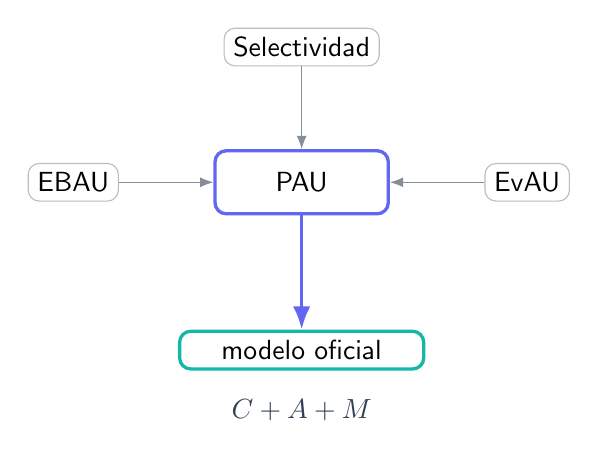
\begin{tikzpicture}[font=\sffamily,>=Latex,node distance=1.05cm and 1.2cm]
  \node[draw=nebula,very thick,rounded corners=4pt,minimum width=2.2cm,minimum height=.8cm] (pau) {PAU};
  \node[draw=ink!35,rounded corners=4pt,left=of pau] (ebau) {EBAU};
  \node[draw=ink!35,rounded corners=4pt,right=of pau] (evau) {EvAU};
  \node[draw=ink!35,rounded corners=4pt,above=of pau] (sel) {Selectividad};
  \node[draw=spark,very thick,rounded corners=4pt,below=1.45cm of pau,minimum width=3.1cm] (model) {modelo oficial};
  \draw[->,ink!60] (sel)--(pau);
  \draw[->,ink!60] (ebau)--(pau);
  \draw[->,ink!60] (evau)--(pau);
  \draw[->,very thick,nebula] (pau)--(model);
  \node[below=7pt of model,text=ink] {$C+A+M$};
\end{tikzpicture}
\end{document}
